\section{Explicit construction of all five solids}
\label{sec:existence}

The upper bound becomes an exact count only after the five possibilities
have been constructed.  We now give coordinates, prove that the displayed
faces are \emph{all} the facets, and verify their regularity and the vertex
valences.  The argument is finite algebra throughout.

Put
\[
 \varphi=\frac{1+\sqrt5}{2},\qquad
 \psi=\varphi-1=\frac1\varphi.
\]
The identities and inequalities used below are
\begin{equation}\label{eq:golden-identities}
 \varphi^2=\varphi+1,\quad
 \psi^2=1-\psi=2-\varphi,\quad
 \varphi\psi=1,\quad
 0<\psi<1<\varphi<2.
\end{equation}
Every coordinate lies in the decidably ordered field $\Q(\varphi)$.
All signs in a coordinate list are independent.  For a set of triples,
$\cyc$ means closure under the three cyclic coordinate permutations
$(x,y,z)$, $(y,z,x)$ and $(z,x,y)$, not under all six permutations.
Define the following finite vertex sets:
\begin{align*}
 T={}&\{(1,1,1),(1,-1,-1),(-1,1,-1),(-1,-1,1)\},\\
 C={}&\{(\pm1,\pm1,\pm1)\},\\
 O={}&\{(\pm1,0,0),(0,\pm1,0),(0,0,\pm1)\},\\
 I={}&\cyc\{(0,\pm1,\pm\varphi)\},\\
 D={}&C\ \cup\ \cyc\{(0,\pm\varphi,\pm\psi)\}.
\end{align*}
Our solids are $\conv(T),\conv(C),\conv(O),\conv(I),\conv(D)$.
The two golden-ratio coordinate sets have been placed in mutually dual
orientations; this will make both facet lists especially simple.

Each hull is three-dimensional.  Subtracting $(1,1,1)$ from the other
three vertices of $T$ gives determinant $-16$.  The set $C$ contains $T$,
the set $O$ contains the three coordinate unit vectors and their negatives,
and $D$ contains $C$.  For $I$, the vectors
\[
 (0,1,\varphi),\quad (1,\varphi,0),\quad (\varphi,0,1)
\]
have determinant $-2\varphi^2\ne0$, and their negatives also belong to $I$.
Within each displayed set, all vertices have the same positive squared
norm.  Distinct points $v,w$ of such a set satisfy
\[
 v\mathbin{\cdot}w
   =\lVert v\rVert^2-\tfrac12\lVert v-w\rVert^2
   <\lVert v\rVert^2.
\]
Thus the functional $x\mapsto v\cdot x$ uniquely exposes $v$.
In particular every displayed point really is a vertex, so counting the
coordinate lists gives the vertex counts without any hidden redundancy.

\begin{figure}[p]
 \centering
 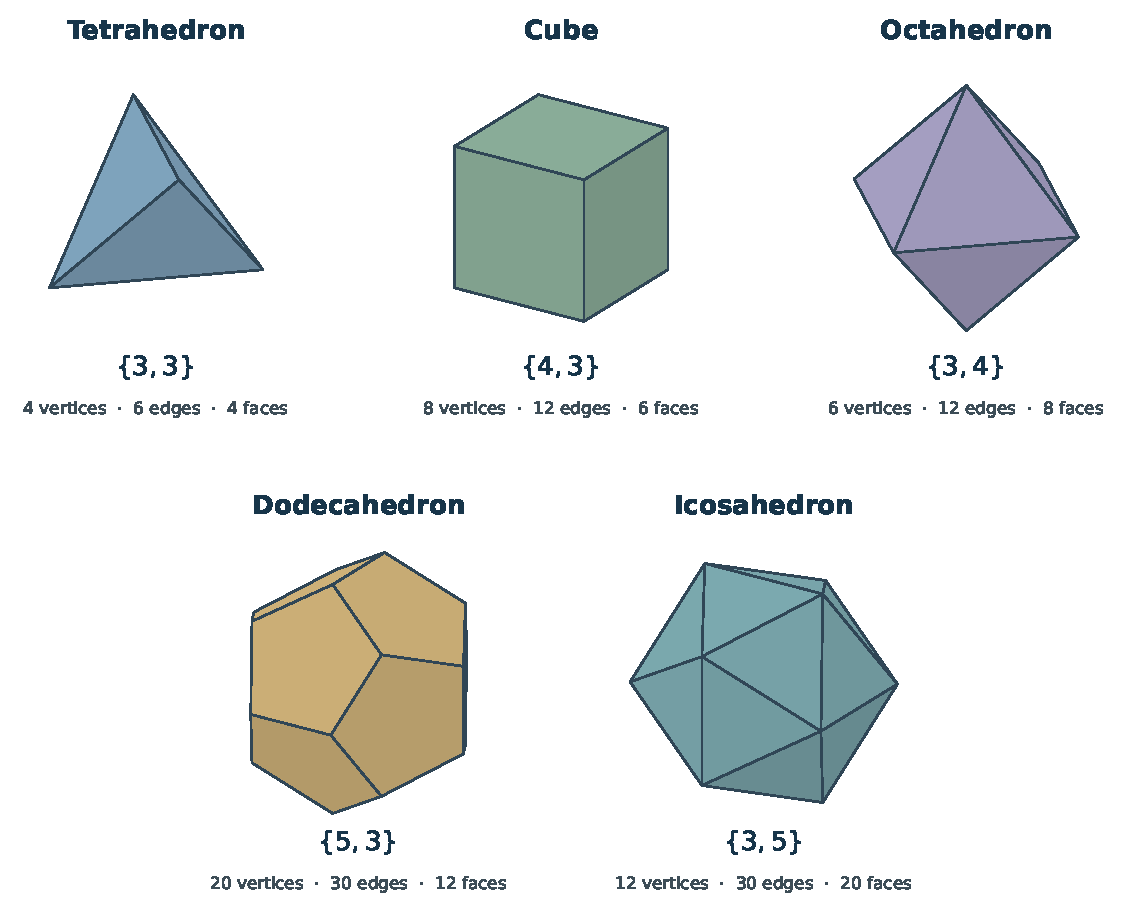
\includegraphics[width=0.97\linewidth]{platonic_models.pdf}
 \caption{The five exact coordinate constructions, rescaled separately
 to a common circumradius for this orthographic illustration.  The
 Schl\"afli symbol $\{p,q\}$ records $p$ edges per face and $q$ faces
 at each vertex.  The coordinates, facet lists and incidence counts
 are established algebraically in this section.}
 \label{fig:five-models}
\end{figure}

\subsection{A finite criterion for a complete facet list}

A facet of a three-dimensional finite convex hull contains three
affinely independent vertices and is the maximizing set of a nonzero
linear functional.  For the present coordinate sets, the normal can
always be chosen in $\Q(\varphi)^3$: take the cross product of two
differences of such facet vertices, and choose its supporting
orientation.  Consequently, all normal-sign cases below are decidable
algebraic cases.  They do not use trichotomy for arbitrary real numbers,
even when the resulting polytope is interpreted in $\R^3$.

This observation also gives a bounded verification procedure: examine
all vertex triples, discard collinear triples, and retain those planes
whose remaining vertices lie on one side.  However, the proof below
does not leave facet completeness to this procedure.  It explicitly
classifies the possible maximizing sets.

\subsection{Tetrahedron, cube and octahedron}

Write the four elements of $T$ as $v_0,v_1,v_2,v_3$.
Their squared norms are $3$, and $v_i\cdot v_j=-1$ for $i\ne j$.
The facet opposite $v_i$ therefore lies in
\[
 (-v_i)\cdot x=1;
\]
the other three vertices attain $1$, whereas $v_i$ gives $-3$.
The four vertices are affinely independent.  Every facet contains at
least three of them, so these four triangles are the complete facet list.
Every pair of distinct vertices has squared distance $8$; the faces are
congruent equilateral triangles.  Each vertex lies on exactly three
faces.  This constructs $\{3,3\}$ with $(V,E,F)=(4,6,4)$.

For $C$, a functional with normal $(a,b,c)$ is maximized by choosing the
sign of each vertex coordinate to agree with the corresponding nonzero
normal coordinate.  A vertex sign is free precisely where that normal
coordinate is zero.  A two-dimensional maximizing set therefore occurs
exactly when the normal has one nonzero coordinate.  The six facets are
\[
 x_i=1\quad\hbox{or}\quad x_i=-1\qquad(1\le i\le3).
\]
Each is a square of side $2$, and three meet at every vertex.
This constructs $\{4,3\}$ with $(V,E,F)=(8,12,6)$.

For $O$, the maximum of the same functional is
$\max(|a|,|b|,|c|)$.  To have three affinely independent maximizing
vertices, all three absolute values must be equal and nonzero.
Thus the eight facets have equations
\[
 s x_1+t x_2+u x_3=1,
 \qquad s,t,u\in\{-1,1\},
\]
and respective vertices $s e_1,t e_2,u e_3$.
Every such triangle is equilateral with squared side length $2$.
At a fixed vertex, one of the three signs is fixed and the other two
are free, so four faces meet there.  This constructs $\{3,4\}$ with
$(V,E,F)=(6,12,8)$.

\subsection{The icosahedron: twenty equilateral facets}

The set $I$ is invariant under independent coordinate sign changes and
cyclic coordinate permutations.  We can therefore take a supporting
normal to be $(a,b,c)$ with $a,b,c\ge0$.  If one coordinate is zero,
a cyclic permutation moves it to the first position.  The maximum of
this functional on $I$ is
\begin{equation}\label{eq:ico-maxima}
 \max(L_1,L_2,L_3),\qquad
 L_1=b+\varphi c,\quad
 L_2=a+\varphi b,\quad
 L_3=\varphi a+c.
\end{equation}

Suppose first that $a,b,c>0$.  Each $L_i$ corresponds to just one
candidate vertex.  A facet requires at least three maximizing vertices,
so $L_1=L_2=L_3$.  The first two equalities give
\[
 a=\varphi c-\psi b,
 \qquad \varphi b=\psi a+c.
\]
Substitution and $\varphi\psi=1$ give
\[
 (\varphi+\psi^2)b=2c.
\]
Since $\varphi+\psi^2=2$, we obtain $b=c$, and then $a=b$.
The facet normal is proportional to $(1,1,1)$.  Restoring signs gives
eight normals of the form $(\pm1,\pm1,\pm1)$.

Next suppose that $a=0$ and $b,c>0$.  Then
$L_3=c<L_1$.  The candidate for $L_1$ is $(0,1,\varphi)$, while
$L_2=\varphi b$ has two candidate vertices $(1,\varphi,0)$ and
$(-1,\varphi,0)$.  There are three maximizing vertices exactly when
\[
 b+\varphi c=\varphi b,
 \qquad\hbox{equivalently}\qquad b=\varphi^2 c.
\]
Its normal is proportional to $(0,\varphi,\psi)$.
Restoring signs and cyclic positions gives twelve more facet normals.
Finally, if two normal coordinates vanish, precisely two vertices
maximize the functional, so its maximizing set is an edge, not a facet.

We have proved that the complete list of supporting facet planes is
\begin{equation}\label{eq:ico-facets}
 n\cdot x=\varphi^2\qquad(n\in D).
\end{equation}
For $n=(1,1,1)$ the maximizing triangle is
\[
 (0,1,\varphi),\quad (1,\varphi,0),\quad (\varphi,0,1).
\]
For $n=(0,\varphi,\psi)$ it is
\[
 (0,1,\varphi),\quad (1,\varphi,0),\quad (-1,\varphi,0).
\]
These cover the two normal orbits under the displayed coordinate
symmetries.  The squared distances between adjacent listed points are
$4$, using
\[
 1+\psi^2+\varphi^2=4;
\]
the edge from $(1,\varphi,0)$ to $(-1,\varphi,0)$ visibly has squared
length $4$ as well.  Thus all twenty facets are congruent equilateral
triangles of side $2$.

The signed cyclic coordinate symmetries act transitively on the twelve
vertices of $I$.  At $(0,1,\varphi)$, the normals from
\eqref{eq:ico-facets} attaining equality are exactly
\[
 (1,1,1),\quad(-1,1,1),\quad(0,\varphi,\psi),\quad
 (\psi,0,\varphi),\quad(-\psi,0,\varphi).
\]
There are five, so every vertex has valence five.
Counting the three edges of every triangle, with each edge counted
twice, gives $2E=3\cdot20$ and hence $E=30$.
This constructs $\{3,5\}$ with $(V,E,F)=(12,30,20)$.

\subsection{The dodecahedron: twelve regular pentagonal facets}

The set $D$ has the same signed cyclic coordinate symmetries.
For a normal $(a,b,c)$ with $a,b,c\ge0$, the maximum on $D$ is
\begin{equation}\label{eq:dodeca-maxima}
 \max(M_0,M_1,M_2,M_3),
 \quad
 \begin{aligned}
 M_0&=a+b+c, & M_1&=\varphi b+\psi c,\\
 M_2&=\varphi a+\psi b, & M_3&=\psi a+\varphi c.
 \end{aligned}
\end{equation}

If $a,b,c>0$, each expression has a unique candidate vertex.
We show that three of them cannot maximize simultaneously.
If $M_0=M_1=M_2$, then
\[
 a=\psi b-\psi^2 c,
 \qquad c=\psi a-\psi^2 b.
\]
Substitution gives $c=-\psi^3c$, impossible because $c>0$.
Cyclic symmetry treats the other two choices involving $M_0$ and two
noncube candidates.  If instead $M_1=M_2=M_3\ge M_0$, their sum would
be at least $3M_0$.  But their actual sum is
\[
 (\varphi+\psi)(a+b+c)<3(a+b+c)=3M_0,
\]
again impossible.  Consequently no facet has an all-positive normal.

Let $a=0$ and $b,c>0$.  We have $M_2=\psi b<M_0$.
Set $t=b-\psi c$.  The two remaining comparisons are particularly
simple:
\[
 M_1-M_0=\psi t,\qquad M_0-M_3=t.
\]
If $t>0$, only $M_1$ maximizes and there is one maximizing vertex.
If $t<0$, only $M_3$ maximizes and the zero first coordinate of the
normal permits two maximizing vertices.
If $t=0$, the maximizing vertices are exactly
\begin{equation}\label{eq:pentagon-vertices}
 \begin{aligned}
 A&=(1,1,1), & B&=(0,\varphi,\psi), & C'&=(-1,1,1),\\
 D'&=(-\psi,0,\varphi), & E'&=(\psi,0,\varphi).
 \end{aligned}
\end{equation}
The normal is proportional to $(0,1,\varphi)$.
Restoring signs and cyclic positions gives twelve facet normals.
When two normal coordinates vanish, only two vertices maximize,
so this last case contributes no further facets.
The complete facet list is therefore
\begin{equation}\label{eq:dodeca-facets}
 n\cdot x=\varphi^2\qquad(n\in I).
\end{equation}

Here is an entirely algebraic verification that the five vertices in
\eqref{eq:pentagon-vertices} form a regular pentagon.
Let $(v_0,v_1,v_2,v_3,v_4)=(A,B,C',D',E')$, with indices taken modulo
five, and put $n=(0,1,\varphi)$.
Substitution in \eqref{eq:golden-identities} gives
\begin{align}
 \lVert v_{i+1}-v_i\rVert^2&=4\psi^2,
 &\lVert v_{i+2}-v_i\rVert^2&=4,
 \label{eq:pentagon-distances}\\
 n\cdot\bigl((v_{i+1}-v_i)\mathbin{\times}(v_{i+r}-v_i)\bigr)
 &=
 \begin{cases}
  6-2\varphi,&r=2,4,\\
  4\varphi-2,&r=3.
 \end{cases}
 \label{eq:pentagon-orientation}
\end{align}
For example,
\[
 \lVert B-A\rVert^2
 =1+\psi^2+\psi^4
 =8-4\varphi=4\psi^2,
 \qquad \lVert C'-A\rVert^2=4.
\]
All values in \eqref{eq:pentagon-orientation} are positive, so every
other vertex lies strictly on the same side of each oriented side
$v_iv_{i+1}$.  Thus the displayed order is the convex boundary order;
in particular it is not a star-polygon ordering.

By \eqref{eq:pentagon-distances}, cyclic shift preserves every pairwise
distance.  A distance-preserving assignment of three noncollinear
points extends uniquely to an isometry of their plane: subtract one
point, use its two independent difference vectors as a basis, and
compare their Gram matrices.  The distances to those three points then
determine every remaining point uniquely in the plane, so this isometry
sends each $v_i$ to $v_{i+1}$.
Its fifth power fixes three noncollinear points and hence is the
identity, while the isometry itself is nontrivial.
It preserves the centroid, has order five, and therefore is an
orientation-preserving plane rotation.  Together with the convex
boundary order, this proves that the facet is a regular pentagon.
This argument uses only finite dot products and nonzero determinants;
no trigonometric functions or limiting argument are required.

All normals in $I$ are carried to one another by the signed cyclic
coordinate symmetries, which preserve $D$.  Hence all twelve
pentagonal facets are congruent.
There are two vertex orbits to check for valence.  At $(1,1,1)$ the
incident facet normals are
\[
 (0,1,\varphi),\quad(1,\varphi,0),\quad(\varphi,0,1).
\]
At $(0,\varphi,\psi)$ they are
\[
 (0,1,\varphi),\quad(1,\varphi,0),\quad(-1,\varphi,0).
\]
The complete normal list \eqref{eq:dodeca-facets} shows that these
lists are exhaustive.  Thus precisely three faces meet at every
vertex.  Counting the five sides of the twelve facets gives
$2E=5\cdot12$, so $E=30$.
This constructs $\{5,3\}$ with $(V,E,F)=(20,30,12)$.

\subsection{Existence certificates and distinction of the five types}

For convenient reference, the exact metric data are collected below.
Here $\ell$ is the common edge length and $R$ the circumradius of the
coordinate model as written; the models have not been normalized to a
common edge length.
\begin{center}
\begin{tabular}{lcccc}
\hline
Solid & $\{p,q\}$ & $(V,E,F)$ & $\ell^2$ & $R^2$\\
\hline
Tetrahedron  & $\{3,3\}$ & $(4,6,4)$   & $8$ & $3$\\
Cube         & $\{4,3\}$ & $(8,12,6)$  & $4$ & $3$\\
Octahedron   & $\{3,4\}$ & $(6,12,8)$  & $2$ & $1$\\
Icosahedron  & $\{3,5\}$ & $(12,30,20)$ & $4$ & $\varphi+2$\\
Dodecahedron & $\{5,3\}$ & $(20,30,12)$ & $4\psi^2$ & $3$\\
\hline
\end{tabular}
\end{center}

Every item used in these constructions is finite and exact: coordinate
pairs in $\Q(\varphi)$, dot and cross products, supporting-plane
inequalities, face cycles and incidence lists.  The accompanying
\texttt{exact\_models.py} independently enumerates all supporting
vertex triples, verifies regular face Gram matrices and the complete
incidences, and exports the resulting finite data in
\texttt{certificates.json}.  It additionally checks exact orthogonal
symmetries acting transitively on all incident vertex--edge--face
flags.  These executable checks support the construction and supply
formalization data; the preceding human proof does not assume their
correctness, and their execution is not itself a kernel-checked proof
in $\ipra$.

\begin{proposition}\label{prop:five-examples}
All five pairs
$\{3,3\},\{4,3\},\{3,4\},\{3,5\},\{5,3\}$ have convex
Platonic realizations over $\Q(\varphi)$.  These five realizations are
pairwise nonsimilar.
\end{proposition}
\begin{proof}
The facet, regularity and valence verifications above prove existence.
A similarity preserves extreme vertices, whereas the five vertex counts
are the distinct numbers $4,8,6,12,20$.  No two displayed realizations
can therefore be similar.
\end{proof}
